	\section{Experimental Setup and Materials}
	\label{sec:exSetup}

	The experiments were carried out on WZL shop floor, located in Aachen in Germany, acquiring thermal images by means of high speed infrared camera FLIR SC7600 (with framerate of 328 fps and a resoloution of 640 x 512 pixels), it was equipped with a macro lens 1:1 and FOV 9.6 x 7.7 mm. The test bench works in a way that the tool stays in a fixed position in relation to the camera, keeping the relative distance between tool and camera constant, then the scale factor provided by this setting was 15 $\mu$m/pixel. It allows the metric conversion for future post processing of images.

	\begin{figure}[H]
		\centering
		\captionsetup{justification=centering}
		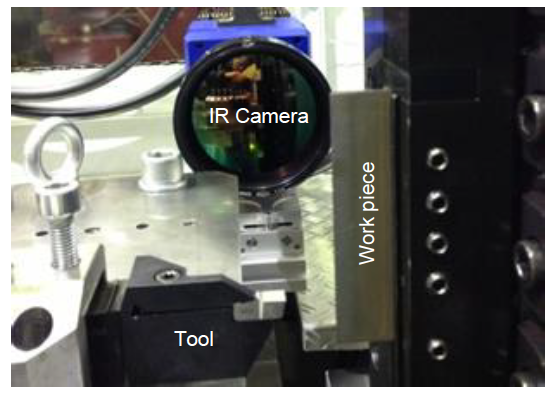
\includegraphics[scale = 0.5]{Cap3/exsetup.png}
		\caption{Experimental setup \cite{augspurger2016experimental}}
		\label{fig:exinfrared}
	\end{figure}

	An important factor for a reliable temperature measurement is the correct choice of the components emissivity. To make it easier, the tool was coated with a black ink, allowing the emissivity valuation for this case, which provided a value of $\epsilon = 0.85$. It is also important to highlight the camera settings, factors as integration time and filters are essential to determine a reliable measurements due to the amount of eletromagnetic radiation received on camera's sensors. The higher are the temperatures higher is the energy produced, then smaller should be the integration time, which is the time that sensor of energy receives radiation and converts into temperature afterwards. These configurations allowed measurements in a range from 200 $^{o}$C until 900 $^{o}$C.
	
	The tool material was uncoated carbide insert (Sandvik H13A), with rake angle 6$^{o}$, clearance angle 3$^{o}$, cutting radius r$_{\beta}$ < 5$\mu$m and width 4.4 mm. The workpiece material was AISI 1045 normalized and its dimensions were 3.5 x 200 x 80 mm (width, lengh, heigth respectively). For the given range of temperature, the thermal conductivity was estimated in $k = 75.4 W/mK$ and for tool heat capaciy was built a regression function ($c(T)$) for corresponding temperature and heat capacity (equations \ref{eq_heatCapTool} and \ref{eq_heatCapWork}).
	
	For force acquisition during the process, it was used a three-component piezoelectric force platform, determining the cutting force and passive force. Since the cutting process is carried out in a linear and constant motion, it is possible to determine the overall power $P$ with velocity and cutting force. From the values obtained of forces along the cutting process it was taken a mean value to be used on power calculation afterwards, equation \ref{eq_power}. 
	
	All the experiments were held without coolant, with cutting velocities of 100 $m/min$ and 150 $m/min$ and a$_{p}$ = [0.2, 0.3, 0.4, 0.5] mm (table \ref{tab:design}).
	The analysis method was built on MATLAB platform with the support of its image processing toolbox. This was the chosen software due the easy connection between FLIR software and MATLAB, since FLIR software can export its images to .mat format, which are indexed matrices prejected to MATLAB environment. Each pixel from the exported images contains information about position and its temperature.

	\begin{table}[H]
		\centering
		\captionsetup{justification=centering}
		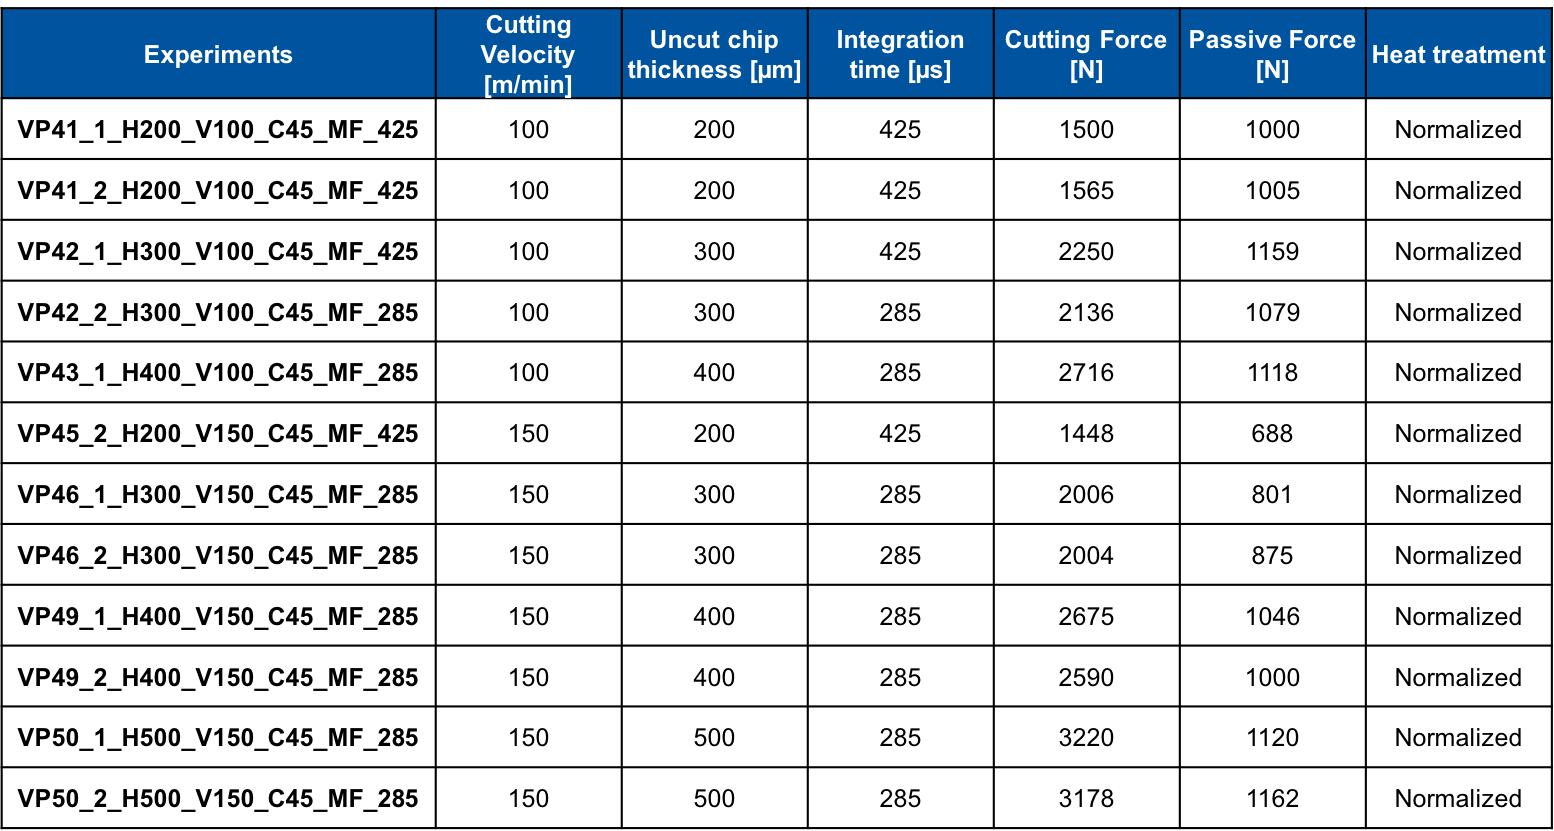
\includegraphics[scale = 0.6]{Cap3/tabexpset.png}
		\caption{Design of experiments \cite{augspurger2016experimental}}
		\label{tab:design}
	\end{table}

	As a machining process, the orthogonal cutting performance is subjected to many parameter like material of workpiece, shape of tool, depth of cut and others. Because of it, the developed algorithm needs the information about all these parameters to work as close as possible of real conditions. Then, all the input data necessary to the  can be summarize on the following table

	\begin{table}[H]
		\centering
		\captionsetup{justification=centering}
		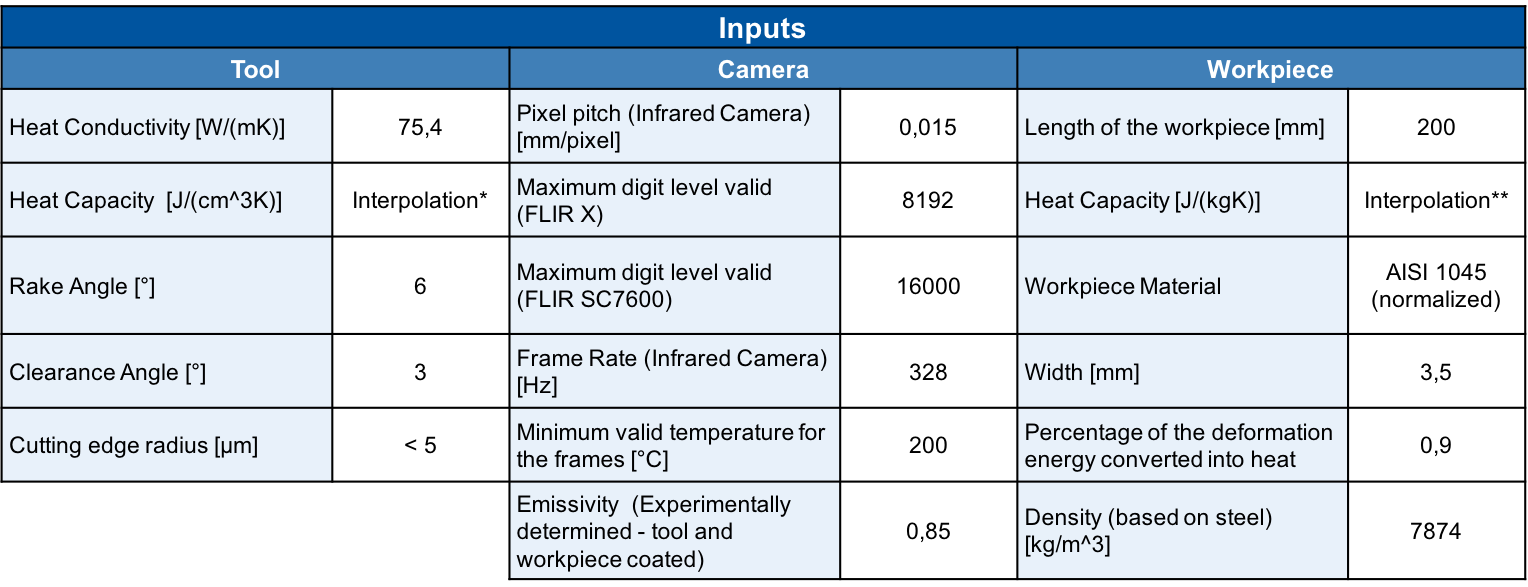
\includegraphics[scale = 0.6]{Imagens/Inputs.png}
		\caption{Algorithm inputs \cite{augspurger2016experimental}}
		\label{tab:inputs}
	\end{table}

	The heat capacities of tool and workpiece material are used as an interpolation function on the code, given by the following equations,

	\begin{equation} 
	\label{eq_heatCapTool}
		c_{p}^{T} = 2.51\times 10^{- 10}\times T^{3} - 1.99\times 10^{- 6} \times T^{2} + 0.0027 \times T + 3.09
	\end{equation}

	\begin{equation} 
	\label{eq_heatCapWork}
		c_{p}^{W} = -4.39\times 10^{- 7}\times T^{3} - 7.07\times 10^{- 4} \times T^{2} + 0.0489 \times T + 481.21
	\end{equation}

	\section{Methods}
	\label{methods}
	
	\subsection{Power calculation}
	This is a known simple method that is stated on the following equation \ref{eq_power}

	\begin{equation} 
	\label{eq_power}
		P = F_{c}v_{c}
	\end{equation}
	
	\subsection{Thermal enegy - chip and tool}
	The methods used in this paper to calculate heat flow through the tool and the energy carried away by chip are based on \cite{boothroyd1963temperatures}.

	\begin{figure}[H]
		\centering
		\captionsetup{justification=centering}
		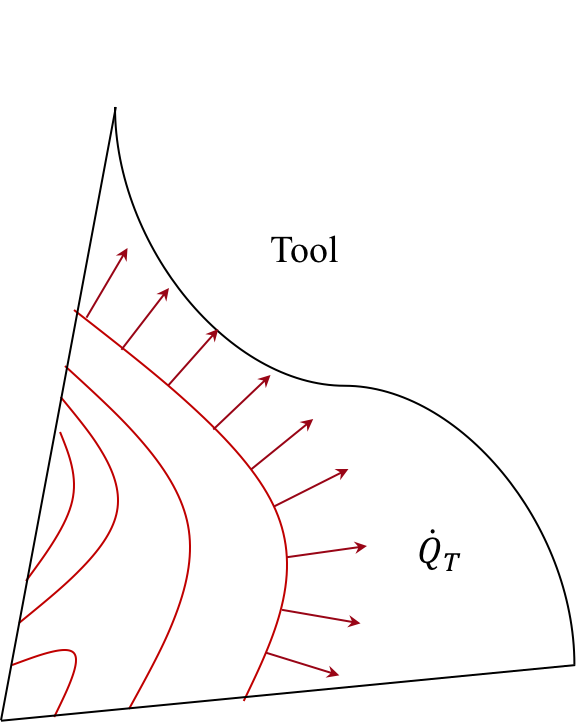
\includegraphics[scale=0.6]{Cap4/ToolHeat.png}
		\caption{Heat flow through tool}
		\label{fig:heattool}
	\end{figure}

	Besides the temperature matrix, it is necessary to calculate heat flow through tool the heat conductivity, the length of the chosen isothermal, the temperature gradient normal to this isothermal and the width of the tool. The calculation is given by the following equation:

	\begin{equation} 
	\label{eq_heattool}
		\dot{Q}_{T} = kL\frac{dT}{dz}w
	\end{equation}

	For the energy carried away by the chip when it flowing through control volume, the variables necessary to calculate this value are the heat capacity function $c_{p}(T)$, the chip temperature distribution along the line where the chip loses contact with tool $T_{C}^{out}$, the environment temperature $T_{e}$, the velocity of chip normal to the line of end of contact $v_{chip}$, the chip thickness $t_{C}$ and the chip width $w$.

	\begin{figure}[H]
		\centering
		\captionsetup{justification=centering}
		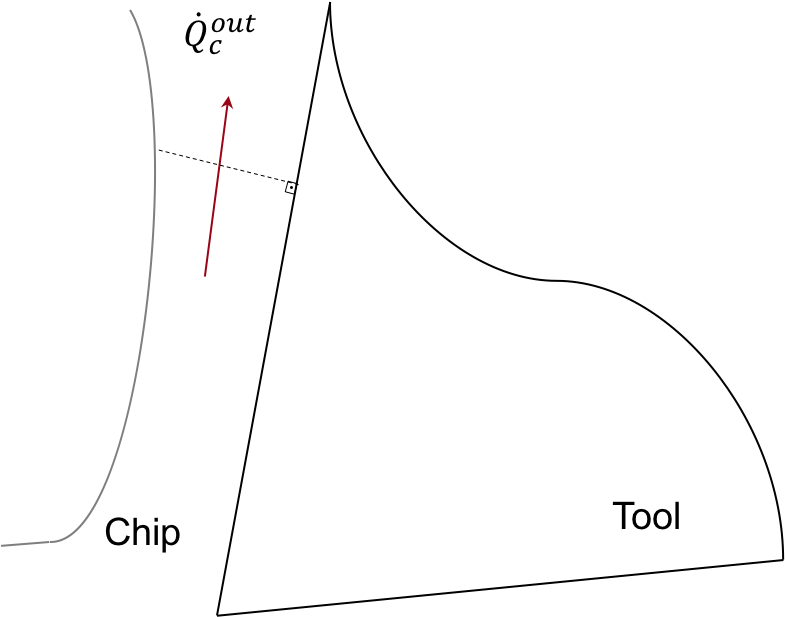
\includegraphics[scale=0.6]{Cap4/energyChip.png}
		\caption{Thermal energy carried away by chip}
		\label{fig:energychip}
	\end{figure}

	The equation for this energy is represented below:

	\begin{equation} 
	\label{eq_energychip}
		\dot{Q}_{C}^{out} = c_{p}^{W}(T_{C}^{out} - T_{e})v_{chip}t_{C}w
	\end{equation}

	That way, having the location and the temperature of each pixel related to the isotherms and the line of end of contact chip - tool, the math necessary to perform these equations is simple, providing reliable outcomes.

	\subsection{Volume control}

	For matter of validation of the presented method and the lack of measurable temperatures on the workpiece surface, it was designed the control volume on figure \ref{fig:volControl}.

	\begin{figure}[H]
		\centering
		\captionsetup{justification=centering}
		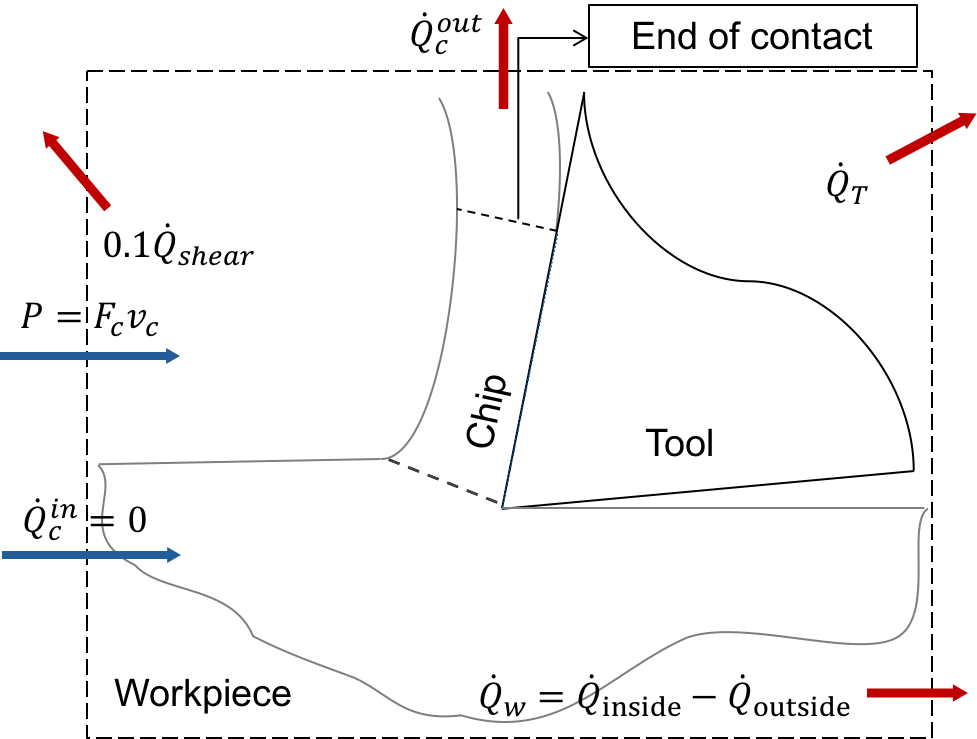
\includegraphics[scale=0.6]{Imagens/volumeControl.png}
		\caption{Control volume}
		\label{fig:volControl}
	\end{figure}

	The shear energy used to raise the temperature of the heat zones is calculated by means of equation \ref{eq_shear}

	\begin{equation} 
	\label{eq_shear}
	\dot{Q}_{shear} = F_{c}v_{c} - F_{p}v_{chip}
	\end{equation}

	It is estimated that $10\%$ of this energy generated in the primary shear zone ($\dot{Q}_{shear}$) is converted into heat and soon dissipated out the control volume(CITAR FONTE AQUI). Then, the energy balance of the control volume will provide:

	\begin{equation} 
	\label{eq_energybalance}
	\dot{Q}_{W} = P - \dot{Q}_{T} - \dot{Q}_{C}^{out} - 0.1\dot{Q}_{shear}
	\end{equation}
